\documentclass{beamer}
\usepackage{amsfonts,amsmath,oldgerm}
\usetheme{sintef}
\usepackage{color}
\usepackage{caption}
\usepackage{subcaption}
\usepackage{biblatex}
\usepackage{framed}

\usepackage{multirow}

\addbibresource{biblio.bib}

\newcommand{\testcolor}[1]{\colorbox{#1}{\textcolor{#1}{test}}~\texttt{#1}}

\usefonttheme[onlymath]{serif}

\titlebackground*{assets/background_BLUE_EPL}

\newcommand{\hrefcol}[2]{\textcolor{cyan}{\href{#1}{#2}}}
\DeclareMathOperator*{\argmax}{argmax}
\DeclareMathOperator*{\argmin}{argmin}
\title{3D change detection to monitor construction sites}

\subtitle{Master [120] in Mathematical / Data Science Engineering}
%\course{Master's Degree in Computer Science}
\author{Dinh Thanh Phong DO \and Nicolas JADOUL}
\date{Academic Year 2022-2023}

%\IDnumber{1234567}

\begin{document}
\maketitle
{
    \begingroup
    \themecolor{main}
    \begin{frame}{Table of Contents}
        \tableofcontents
    \end{frame}
    \endgroup
}
\nocite{*}
\section{Context and Objectives}
\begin{frame}[t,allowframebreaks]
    \frametitle{Context}
    \begin{itemize}
        \item Autonomous navigation in robotic allows new applications
        \item Monitoring construction sites by detecting changes in point cloud records
        \item Our objective is to propose approaches and proof-of-concepts
    \end{itemize}
    \begin{figure}[ht]
        \begin{subfigure}{.48\linewidth}
        \centering
        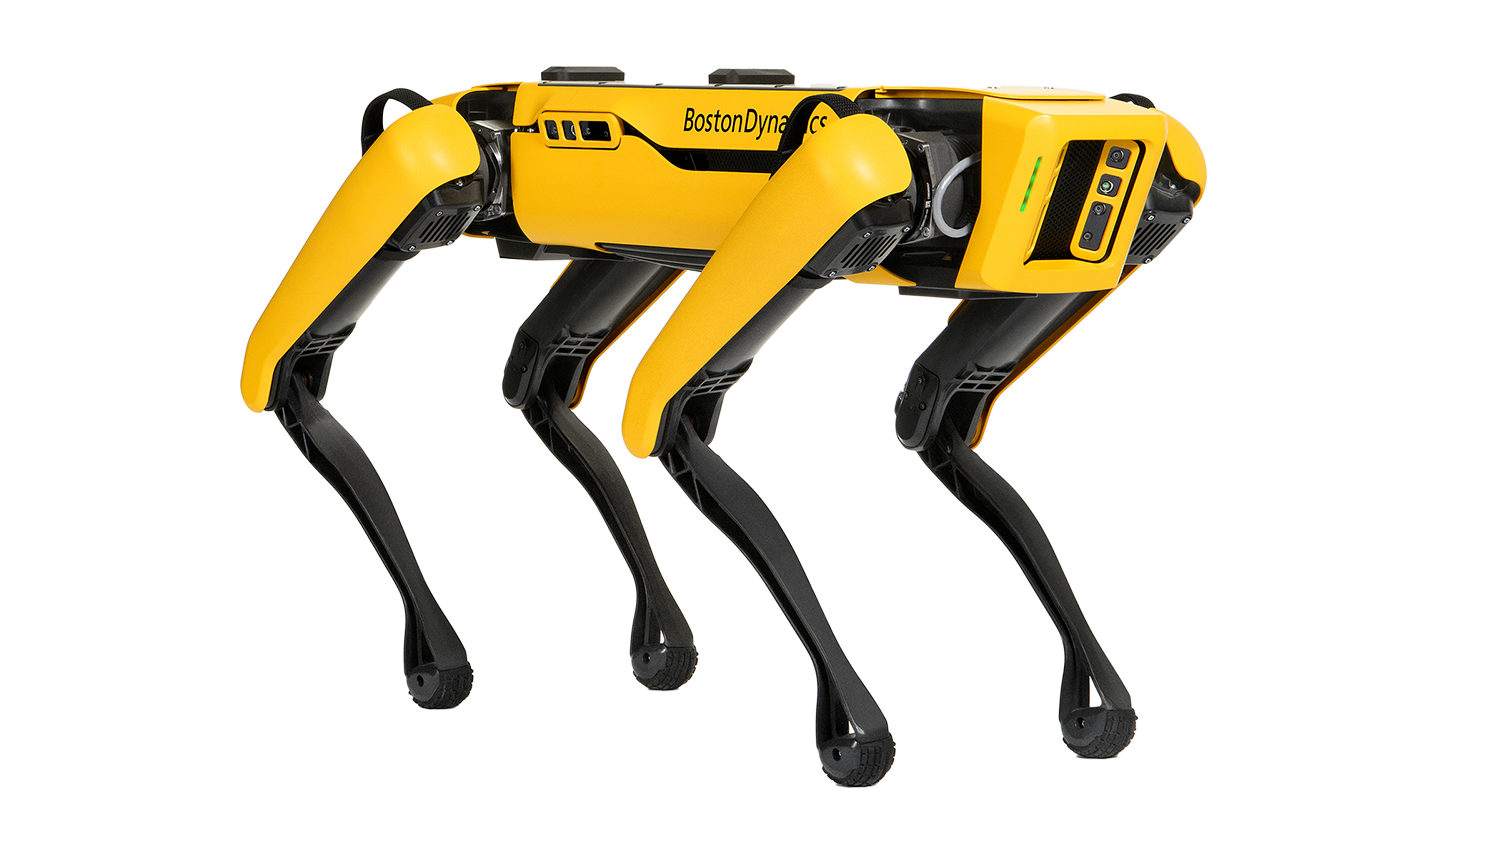
\includegraphics[scale=0.15]{img/spot-explorer-web-sm.png}
        \end{subfigure}
        \begin{subfigure}{0.48\linewidth}
        \centering
        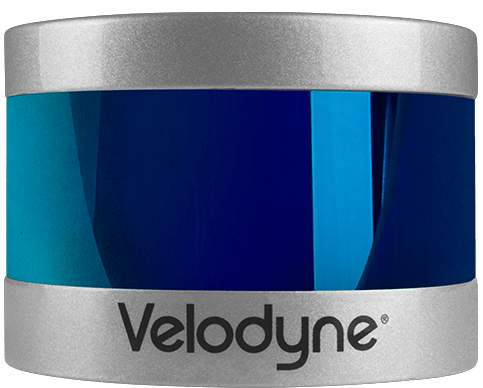
\includegraphics[scale = 0.2]{img/00_VLP-16_1.png}
        \end{subfigure}\\
    \end{figure}
\end{frame}
\begin{frame}[t,allowframebreaks]
% pros and cons
    \frametitle{Our approaches}
    \begin{itemize}
        \item Classical approach:
            \begin{figure}
                \centering
                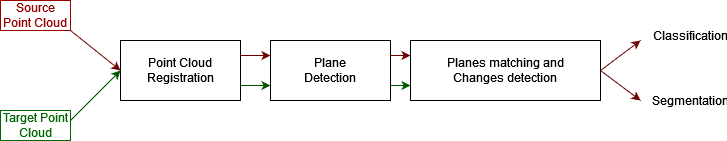
\includegraphics[scale=0.4]{img/approach1.drawio.png}
            \end{figure}
        \item Deep learning approach:
            \begin{figure}
                \centering
                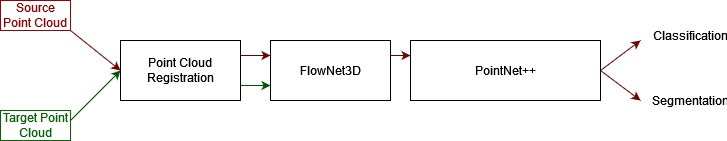
\includegraphics[scale=0.4]{img/approach2.drawio.png}
            \end{figure}
    \end{itemize}
    
    
\end{frame}

\begin{frame}{Point Cloud Registration}
    \begin{itemize}
        \item Result of the registration using pre-built method from Open3D (RANSAC \& ICP) 
    \end{itemize}
    
    \begin{figure}
        \begin{subfigure}{.48\linewidth}
        \centering
        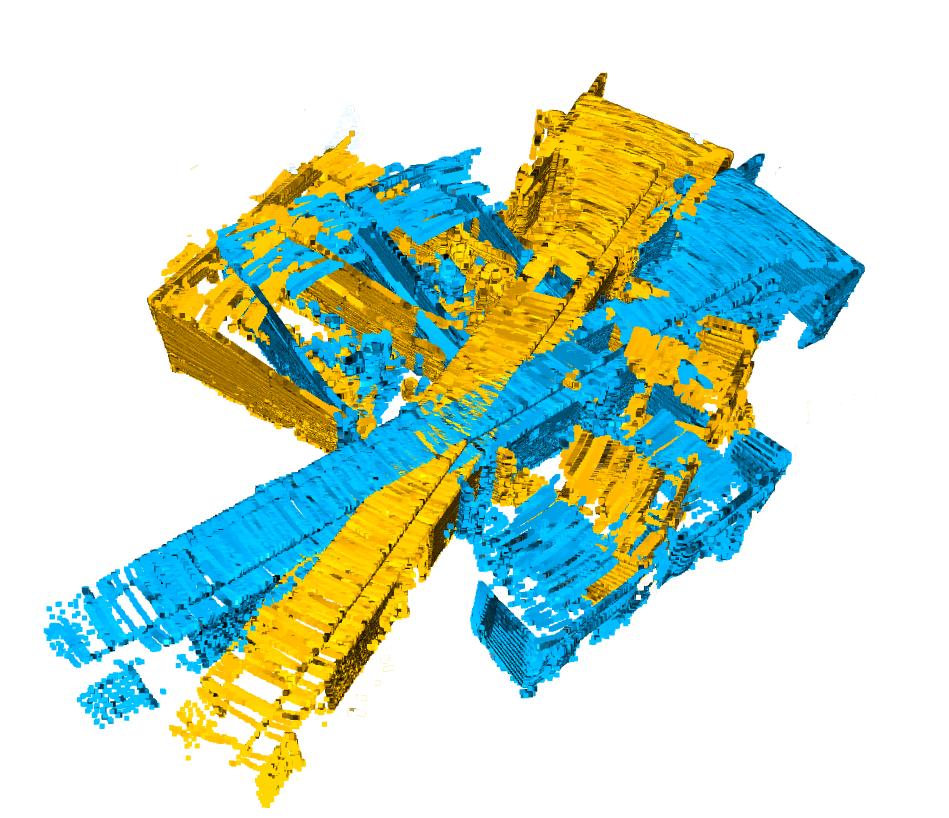
\includegraphics[scale=0.15]{img/06_ICP0.png}
        \end{subfigure}
        \begin{subfigure}{.48\linewidth}
        \centering
        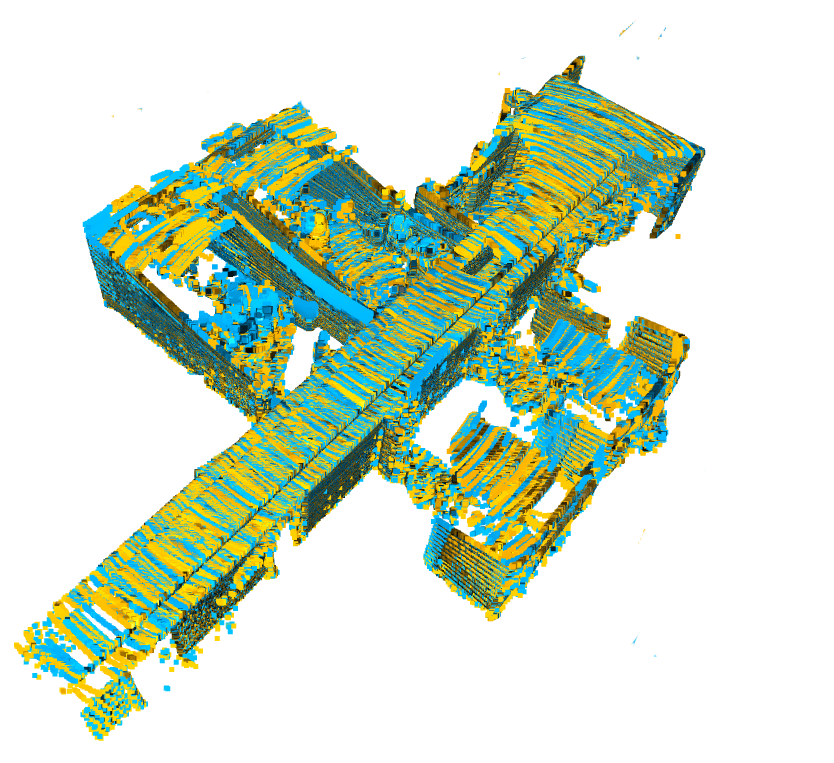
\includegraphics[scale=0.16]{img/06_ICP1.png}
        \end{subfigure}\\
    \end{figure}
\end{frame}

\section{Classical Approach}

\begin{frame}{Planes Detection: RANSAC}
\begin{minipage}{\textwidth}
    \begin{minipage}{0.45\textwidth}
        \begin{itemize}
            \item Select 3 random points to fit a candidate plane.
            \item Determine the number of inliers.
            \item Choose the candidate plane with the most inliers
        \end{itemize}
    \end{minipage}
    \hfill
    \begin{minipage}{0.45\textwidth}
        \begin{figure}
            \centering
            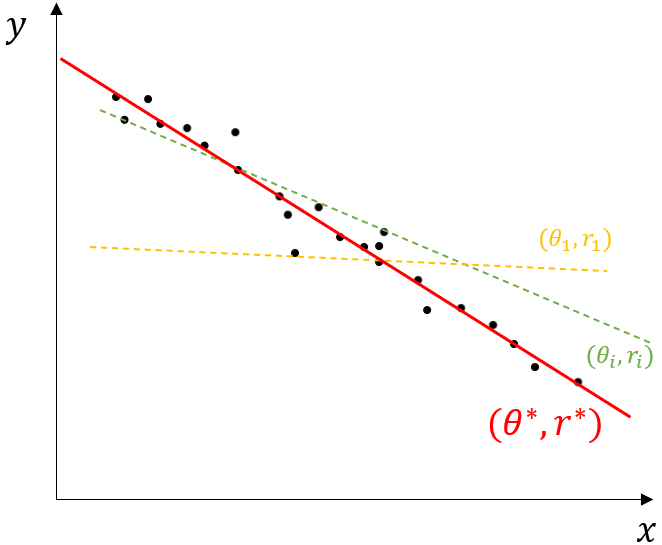
\includegraphics[width=\textwidth,height=0.8\textheight,keepaspectratio]{img/03_RANSAC2.png}
        \end{figure}
    \end{minipage}
\end{minipage}
\end{frame}

\begin{frame}{Planes Matching and Changes Detection}
\begin{enumerate}
    \item Planes Matching:
    \begin{itemize}
        \item Select the most aligned plane when the centroid distance is within a certain range
    \end{itemize}
    \item Change Detection
    \begin{table}[]
        \centering
        \begin{tabular}{|c||c|c|}\hline 
             & Normals are aligned & Centroids are close\\ \hline \hline
             Translation& Yes &  No \\ \hline 
             Unchanged & Yes & Yes \\ \hline
             Rotation & No & Yes/No\\ \hline 
        \end{tabular}
    \end{table}
\end{enumerate}
    
\end{frame}

\section{Deep Learning Approach}
% Only planes -> general structures with DL.
\begin{frame}[b]
    \frametitle{Artificial Neural Network}
    \begin{figure}
    \begin{subfigure}{.48\linewidth}
    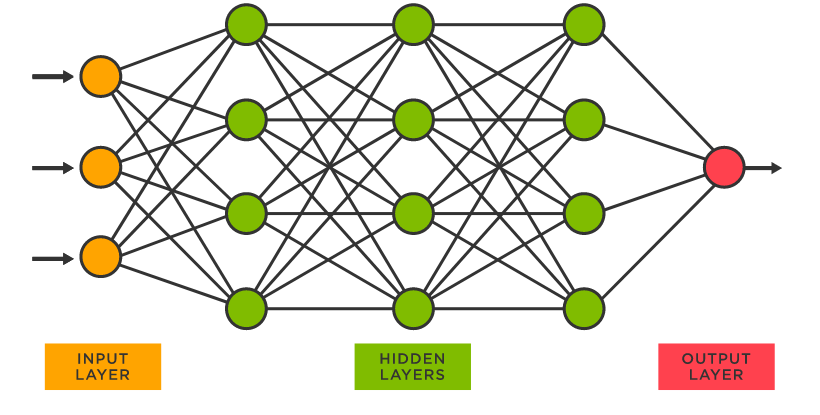
\includegraphics[width = \linewidth]{img/05_ANN.png}
    \caption{Multi-Layer Perceptron (MLP)}
    \end{subfigure}
    \hfill
    \begin{subfigure}{0.48\linewidth}
    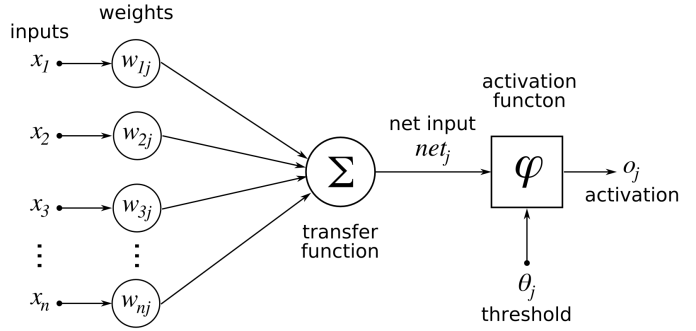
\includegraphics[width = \linewidth]{img/05_Neuron.png}
    \caption{Interaction for a single neuron}
    \end{subfigure}
    \end{figure}

\end{frame} 
\begin{frame}[t,allowframebreaks]
    \frametitle{Our network}
    \begin{figure}
        \centering
        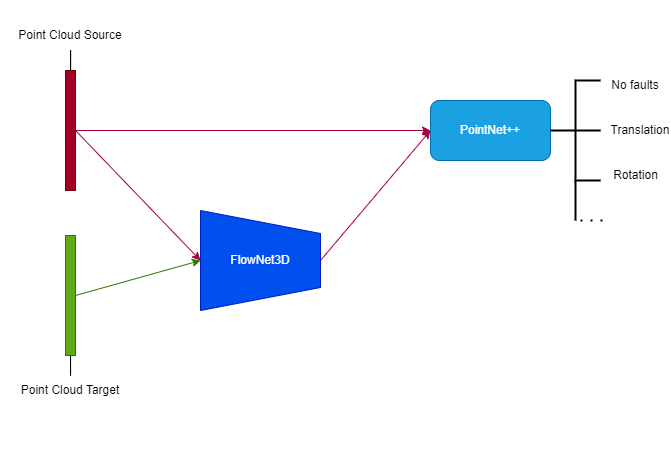
\includegraphics[scale=0.35]{img/05_OurNetwork.png}
        \label{fig:enter-label}
    \end{figure}
\end{frame}
\begin{frame}[t,allowframebreaks]
    \frametitle{PointNet}
     
    \begin{figure}
        \centering
        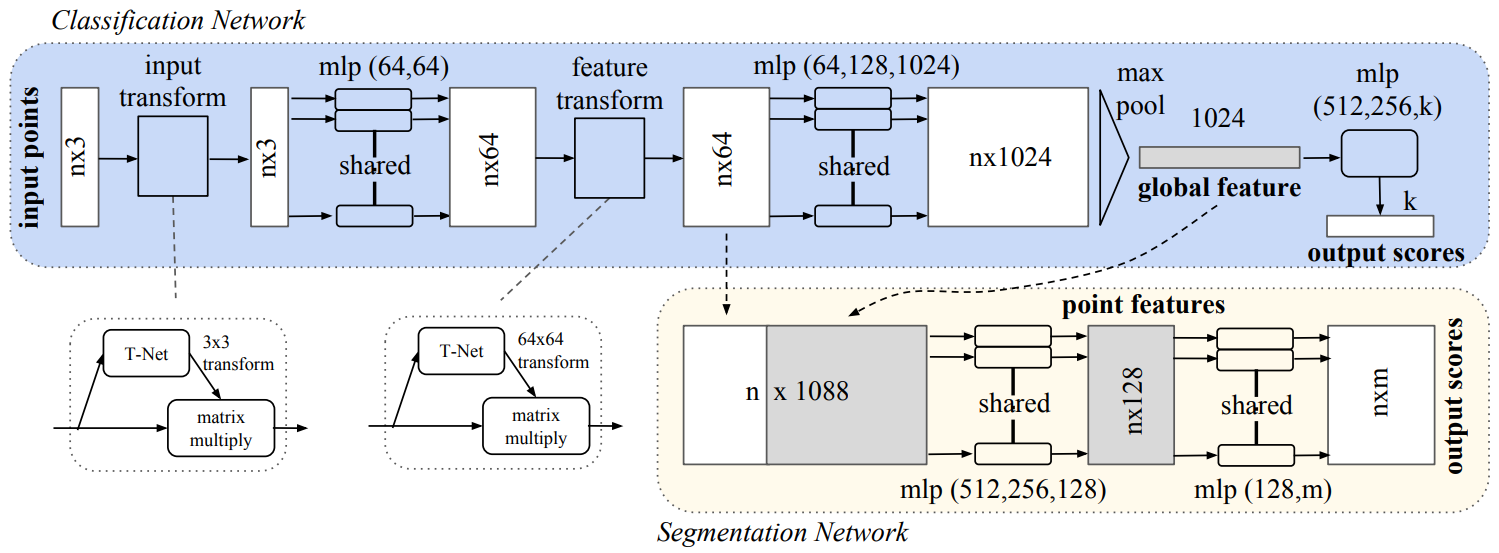
\includegraphics[width=\textwidth,height=0.8\textheight,keepaspectratio]{img/05_Pointnet.png}
        
        \label{fig:enter-label}
    \end{figure}
\end{frame}
\begin{frame}[allowframebreaks]
\frametitle{PointNet: Invariance under transformation}
\begin{minipage}{\textwidth}
    \begin{minipage}{0.45\textwidth}
    \begin{itemize}
        \item \textbf{T-Net}\\
        $\hookrightarrow$ Transformation matrix that projects into a canonical space\\
    \end{itemize}
        
    \end{minipage}
    \hfill
    \begin{minipage}{0.45\textwidth}
        \begin{figure}
        \centering
        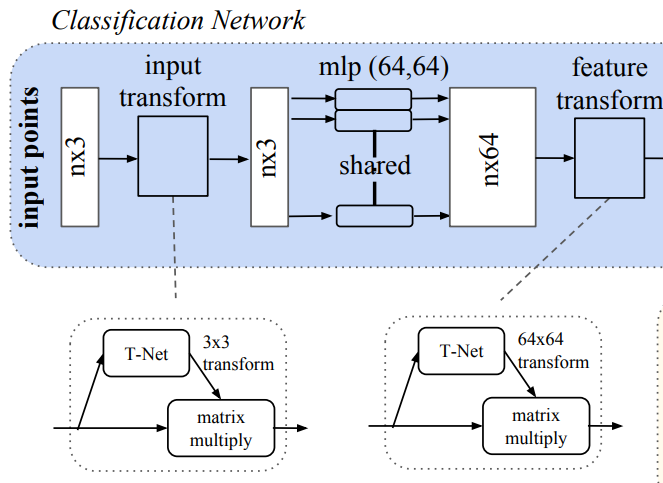
\includegraphics[width=\textwidth,height=0.8\textheight,keepaspectratio]{img/05_Pointnet_JAN.png}
        
        \label{fig:enter-label}
    \end{figure}
    \end{minipage}
\end{minipage}
\end{frame}
\begin{frame}[allowframebreaks]
\frametitle{PointNet: Unordered point clouds}
\begin{minipage}{\textwidth}
\begin{minipage}{0.45\textwidth}
        \begin{figure}
        \centering        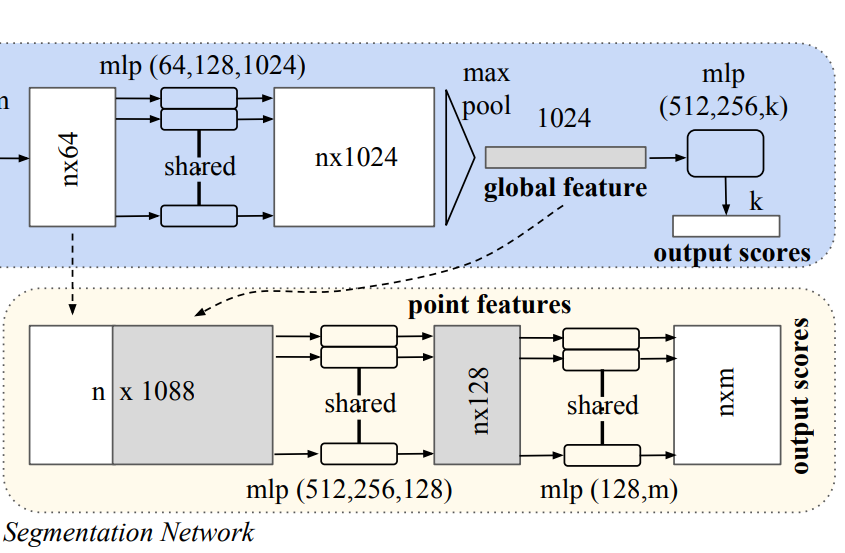
\includegraphics[width=\textwidth,height=0.8\textheight,keepaspectratio]{img/05_Pointnet_end.png}
        
        \label{fig:enter-label}
    \end{figure}
    \end{minipage}
    \hfill
    \begin{minipage}{0.45\textwidth}
        \begin{itemize}
            \item \textbf{Max Pooling}
            \item Classification : global feature
            \item Segmentation : Local + global features
        \end{itemize}
    \end{minipage}
    
    
\end{minipage}
\end{frame}
\begin{frame}[t,allowframebreaks]
    \frametitle{PointNet++}
    \begin{figure}
        \centering
        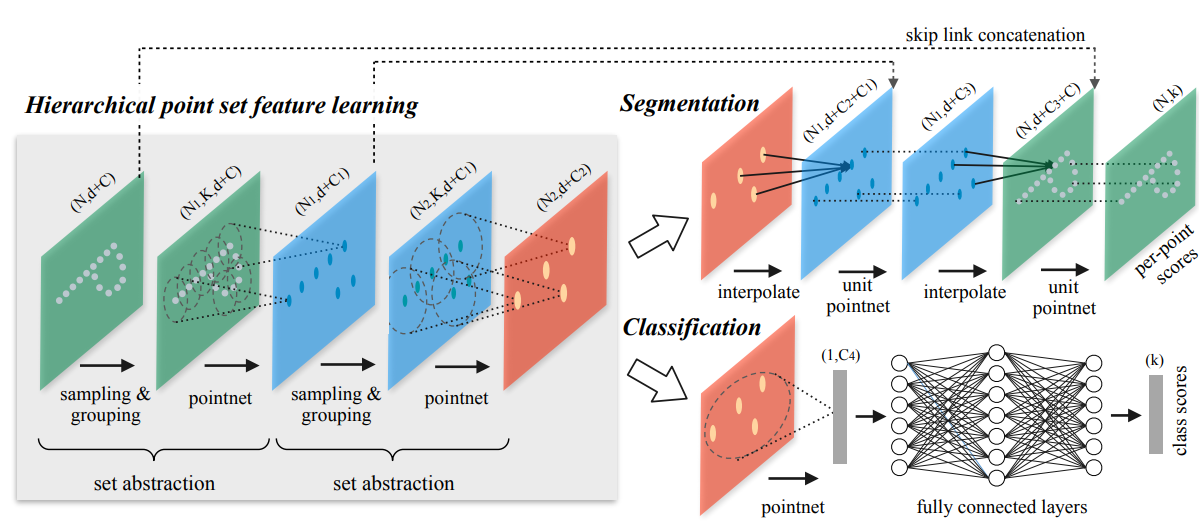
\includegraphics[width=\textwidth,height=0.8\textheight,keepaspectratio]{img/05_Pointnet2.png}
        \label{fig:enter-label}
    \end{figure}
\end{frame}
\begin{frame}[t,allowframebreaks]
    \frametitle{Our network}
    \begin{figure}
        \centering
        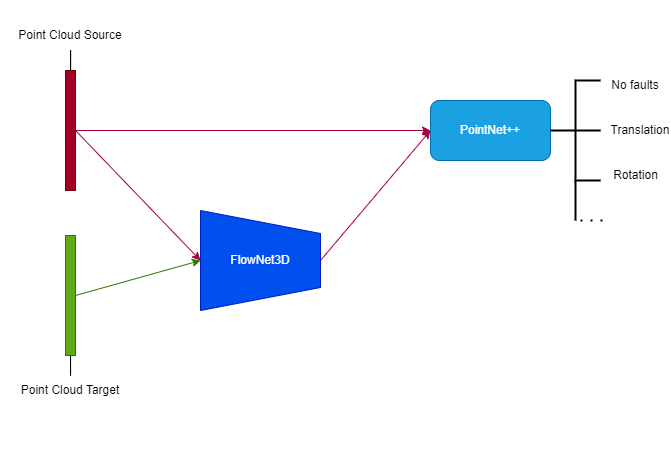
\includegraphics[scale=0.35]{img/05_OurNetwork.png}
        \label{fig:enter-label}
    \end{figure}
\end{frame}
\begin{frame}[t,allowframebreaks]
    \frametitle{FlowNet3D}
    \begin{figure}
        \centering
        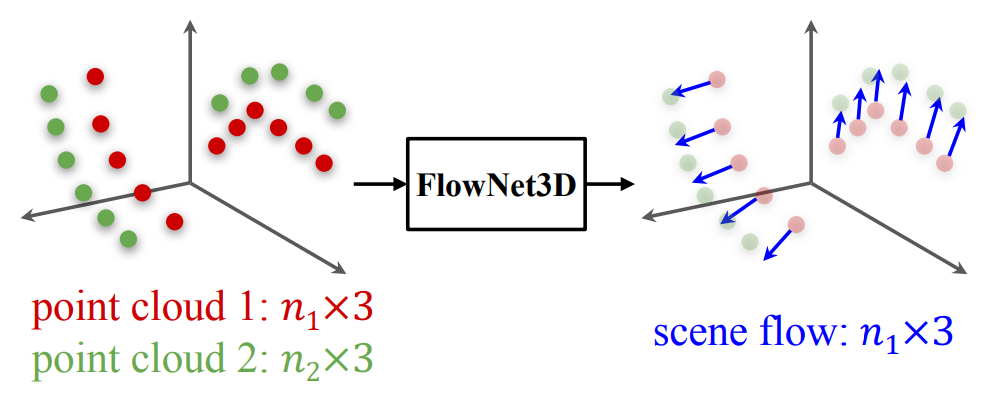
\includegraphics[width=\textwidth,height=0.8\textheight,keepaspectratio]{img/05_Flow3D.png}
        \label{fig:enter-label}
    \end{figure}
    \begin{figure}
        \centering
        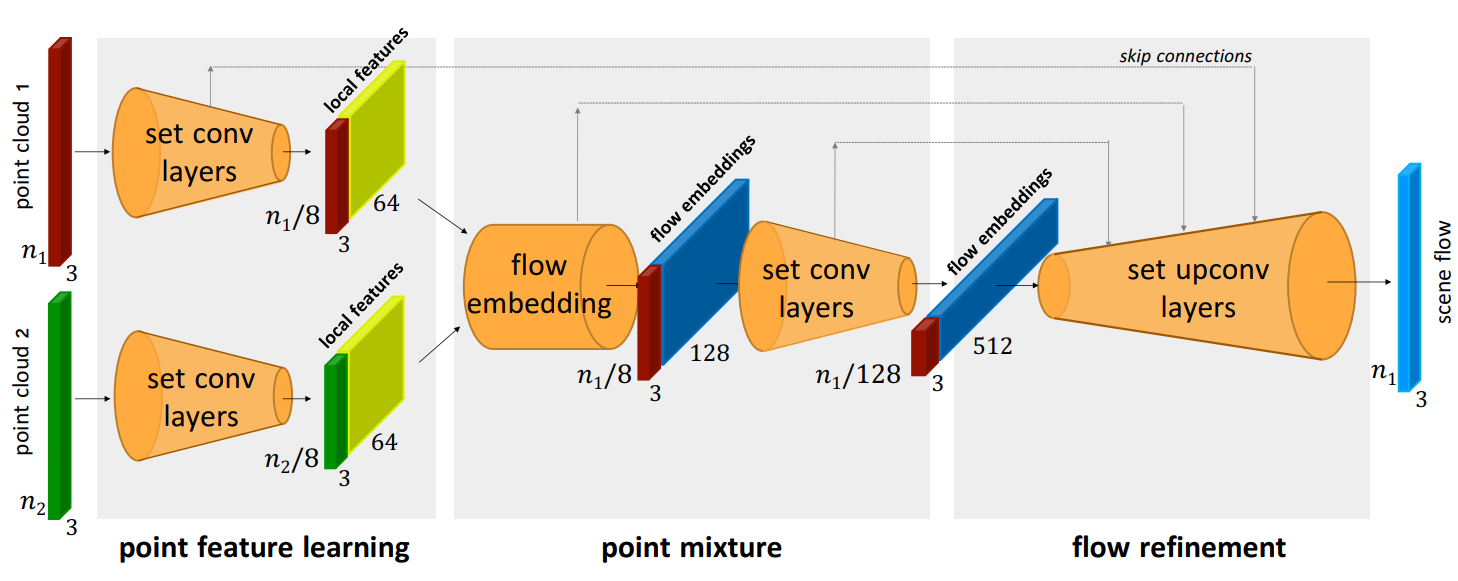
\includegraphics[width=\textwidth,height=0.8\textheight,keepaspectratio]{img/05_FlowNet3D.png}
        \label{fig:enter-label}
    \end{figure}
\end{frame}



\begin{frame}[allowframebreaks]
\frametitle{FlowNet3D : flow embedding}
\begin{minipage}{\textwidth}
\begin{minipage}{0.45\textwidth}
        \begin{figure}
        \centering        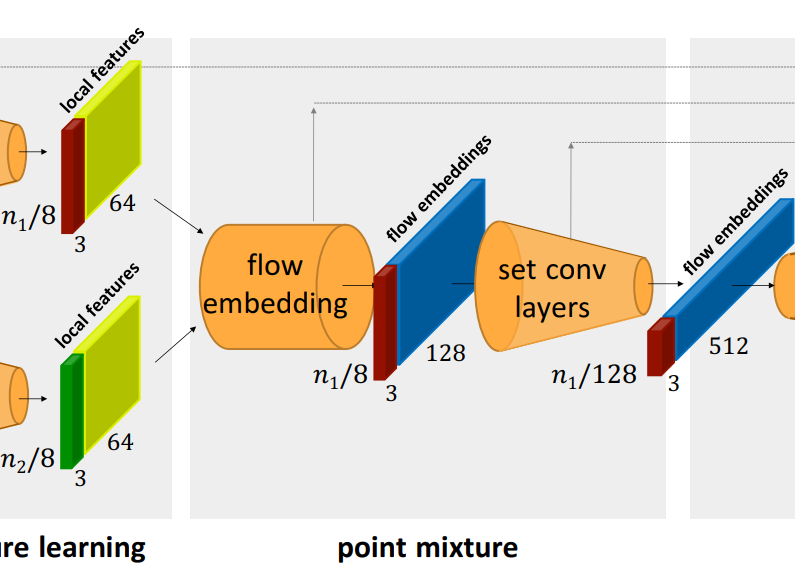
\includegraphics[width=\textwidth,height=0.8\textheight,keepaspectratio]{img/05_FlowNet3D_point_mixture.png}        
        \label{fig:enter-label}
    \end{figure}
    \end{minipage}
    \hfill
    \begin{minipage}{0.45\textwidth}
        \begin{itemize}
            \item Weighted flow vote using features of both point cloud
            \item Conv layers : spatial-smoothing
        \end{itemize}
    \end{minipage} 
\end{minipage}
\end{frame}

\begin{frame}[t,allowframebreaks]
    \frametitle{Our network}
    \begin{figure}
        \centering
        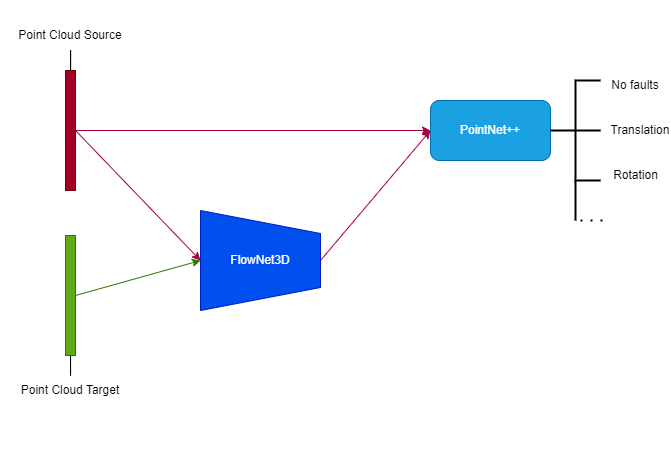
\includegraphics[scale=0.35]{img/05_OurNetwork.png}
        \label{fig:enter-label}
    \end{figure}
\end{frame}

\section{Results}
\begin{frame}{Dataset}
\begin{minipage}{\textwidth}
    \begin{minipage}{0.44\textwidth}
        \begin{itemize}
            \item Classification and Segmentation dataset
            \item Rectangular cuboid models a room
            \item Each wall/plane is assigned to a class:
            \begin{itemize}
                \item Translation
                \item Rotation
                \item Unchanged
            \end{itemize}
            \item Noise $\mathcal{N}(0,\; 0.015)$ meters
        \end{itemize} 
    \end{minipage}
    \hfill
    \begin{minipage}{0.55\textwidth}
        \begin{figure}
            \centering
            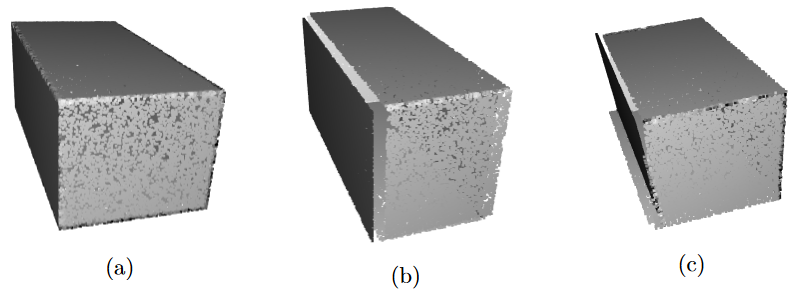
\includegraphics[width = \textwidth]{img/06_rooms.png}
        \end{figure}
    \end{minipage}
\end{minipage}
 \end{frame}

\begin{frame}{Evaluation Metrics}
\begin{minipage}{\textwidth}
    \begin{minipage}{0.6\textwidth}
        \begin{itemize}
            \item Accuracy metric:
                \begin{equation*}
                    \text{Acc} = \frac{TP + TN}{TP + FP + TN + FN}
                \end{equation*}
            \item Intersection over Union (IoU):
                \begin{equation*}
                    \text{IoU} = \frac{\text{Area of Overlap}}{\text{Area of union}} = \frac{TP}{TP+FP+FN}
                \end{equation*}
        \end{itemize}
        
    \end{minipage}
    \hfill
    \begin{minipage}{0.38\textwidth}
        \begin{figure}
            \centering
            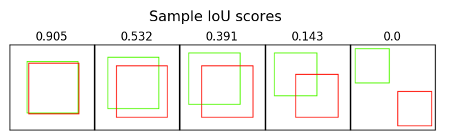
\includegraphics[width = \textwidth]{img/iou_scores.png}
        \end{figure}
        \begin{figure}
            \centering
            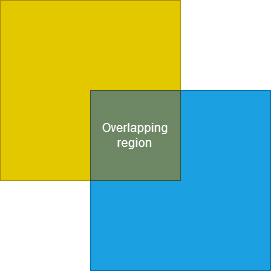
\includegraphics[width = 0.8\textwidth]{img/IoU.drawio.png}
        \end{figure}

    \end{minipage}
\end{minipage}
\end{frame}





\begin{frame}{Comparison between results}
theor. = Theoretical flows\\
pretr. = Flow computed with a pre-trained FlowNet3D
\begin{table}
  \begin{tabular}{|l|l|l|l|l|l|l|l|l|l|}
    \hline

    Classical model &
      \multicolumn{2}{c|}{Unchanged} &
      \multicolumn{2}{c|}{Translation} &
      \multicolumn{2}{c|}{Rotation} &
      \multicolumn{2}{c|}{Average} \\ \hline
    Accuracy &
      \multicolumn{2}{c|}{93.8\%} &
      \multicolumn{2}{c|}{90.5\%} &
      \multicolumn{2}{c|}{60.0\%} &
      \multicolumn{2}{c|}{81.4\%} \\ \hline
    IoU &
      \multicolumn{2}{c|}{72.3\%} &
      \multicolumn{2}{c|}{84.0\%} &
      \multicolumn{2}{c|}{56.6\%} &
      \multicolumn{2}{c|}{71.0\%} \\ \hline \hline
    \multirow{2}{*}{Deep Learning model} &
      \multicolumn{2}{c}{Unchanged} &
      \multicolumn{2}{c}{Translation} &
      \multicolumn{2}{c}{Rotation} &
      \multicolumn{2}{c|}{Average} \\
    & theor. & pretr. & theor. & pretr. & theor. & pretr. & theor. & pretr. \\
    \hline
    Accuracy & 97.2\% & 67.2\% & 88.9\% & 76.2\% & 78.6\% & 20.8\% & 88.2\% & 54.7\% \\
    \hline
    IoU &      88.7\% & 38.6\% & 84.9\% & 51.6\% & 67.4\% & 16.6\% & 80.3\% & 35.6\%\\ \hline
  \end{tabular}
\end{table}
\end{frame}

\begin{frame}{Discussion}
    \begin{itemize}
        \item The DL model with theoretical flows shows promising results
        \item The flows computed with FlowNet3D need to be improved
        \item Rotation class poses greater challenges
    \end{itemize}
    \begin{table}
      \begin{tabular}{|l|l|l|l|l|l|l|l|l|l|}
        \hline
    
        Classical model &
          \multicolumn{2}{c|}{Unchanged} &
          \multicolumn{2}{c|}{Translation} &
          \multicolumn{2}{c|}{Rotation} &
          \multicolumn{2}{c|}{Average} \\ \hline
        Accuracy &
          \multicolumn{2}{c|}{93.8\%} &
          \multicolumn{2}{c|}{90.5\%} &
          \multicolumn{2}{c|}{60.0\%} &
          \multicolumn{2}{c|}{81.4\%} \\ \hline
        IoU &
          \multicolumn{2}{c|}{72.3\%} &
          \multicolumn{2}{c|}{84.0\%} &
          \multicolumn{2}{c|}{56.6\%} &
          \multicolumn{2}{c|}{71.0\%} \\ \hline \hline
        \multirow{2}{*}{Deep Learning model} &
          \multicolumn{2}{c}{Unchanged} &
          \multicolumn{2}{c}{Translation} &
          \multicolumn{2}{c}{Rotation} &
          \multicolumn{2}{c|}{Average} \\
        & theor. & pretr. & theor. & pretr. & theor. & pretr. & theor. & pretr. \\
        \hline
        Accuracy & 97.2\% & 67.2\% & 88.9\% & 76.2\% & 78.6\% & 20.8\% & 88.2\% & 54.7\% \\
        \hline
        IoU &      88.7\% & 38.6\% & 84.9\% & 51.6\% & 67.4\% & 16.6\% & 80.3\% & 35.6\%\\ \hline
      \end{tabular}
    \end{table}
\end{frame}

\begin{frame}{Theoretical flows visualisation}
\begin{minipage}{\textwidth}
    \begin{minipage}{0.3\textwidth}
        \begin{itemize}
            \item Green = translation
            \item Red = rotation
            \item Grey = unchanged
        \end{itemize}
        
    \end{minipage}
    \hfill
    \begin{minipage}{0.7\textwidth}
        \begin{figure}
            \centering
            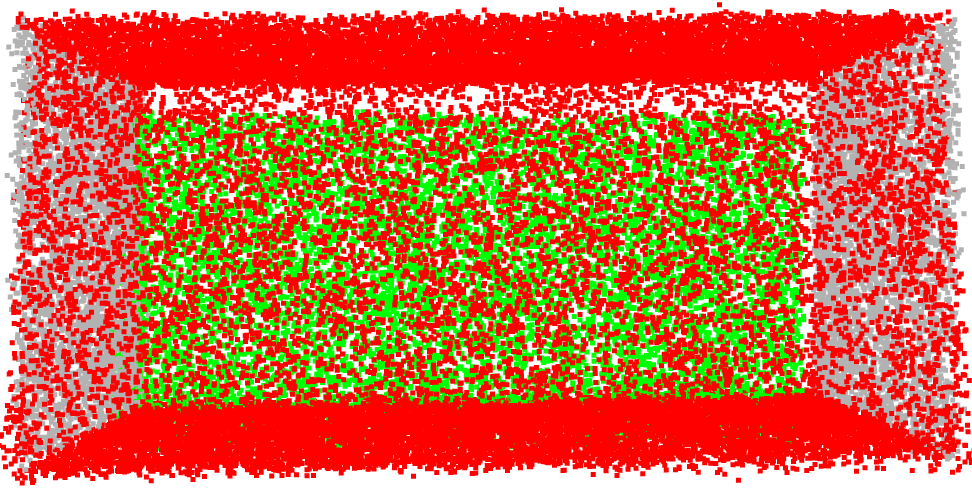
\includegraphics[width = 0.6\textwidth]{img/Results_nogift_clean.png}
        \end{figure}
        \begin{figure}
            \centering
            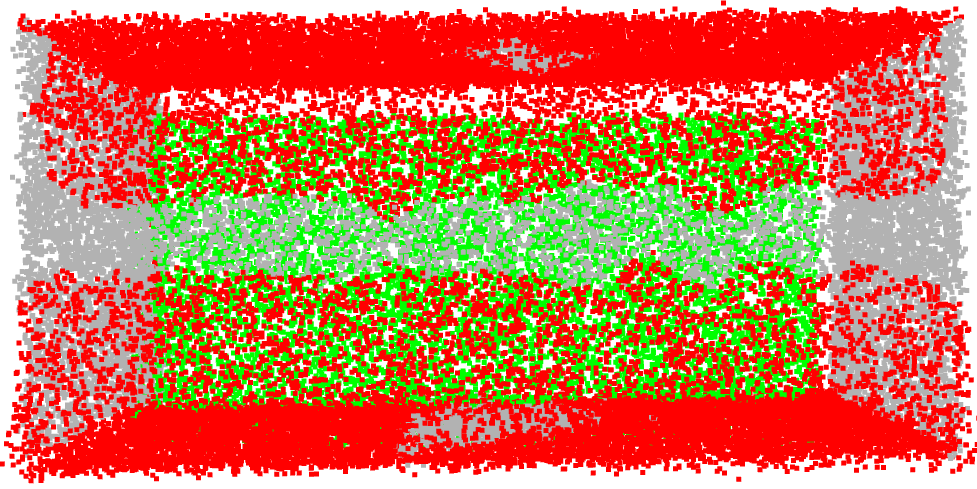
\includegraphics[width = 0.6\textwidth]{img/Results_gift_clean.png}
        \end{figure}
    \end{minipage}
\end{minipage}  
\end{frame}

\section[]{Conclusion}
\begin{frame}{Conclusion}
    \begin{itemize}
        \item Change detection using 2 different approaches
        \item Promising results for the DL model with theoretical flows.
        \item Potential for future improvements:
        \begin{itemize}
            \item Network architecture and training
            \item Real dataset, additional faults
        \end{itemize}
    \end{itemize}
\end{frame}

\backmatter

\section*{References}
\begin{frame}[t,allowframebreaks]
    \frametitle{References}
    \small \printbibliography[heading=none]
\end{frame}
\section*{Backup Slides}

\begin{frame}{Results: Training the Deep learning model}
\begin{minipage}{\textwidth}
    \begin{minipage}{0.66\textwidth}
        \begin{itemize}
            \item Batch Size = 32
            \item Adamgrad optimizer
            \item Blocksize = 3
        \end{itemize}
        
    \end{minipage}
    \hfill
    \begin{minipage}{0.33\textwidth}
        \begin{figure}
            \centering
            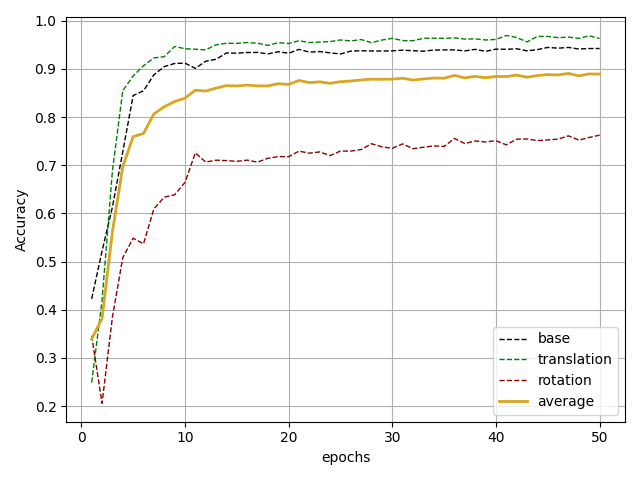
\includegraphics[width = 0.9\textwidth]{img/seg_noise_train_acc.png}
        \end{figure}
        \begin{figure}
            \centering
            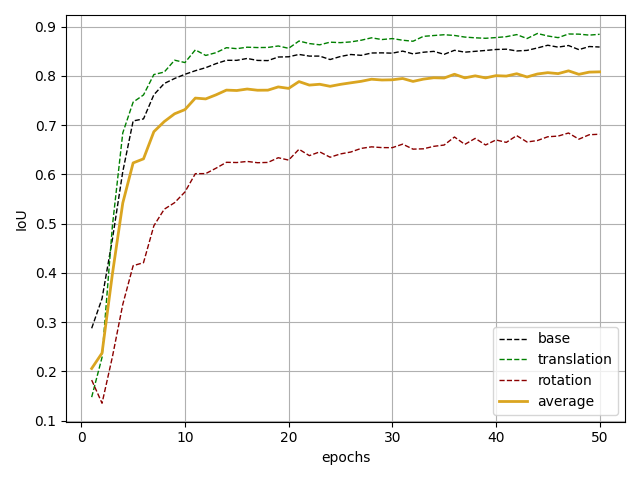
\includegraphics[width = 0.9\textwidth]{img/seg_noise_train_iou.png}
        \end{figure}
    \end{minipage}
\end{minipage}
\end{frame}

\begin{frame}{ICP}
\begin{enumerate}
    \item Let $R \in \mathbb{R}^{3\times 3}$ be a rotation matrix and $t \in \mathbb{R}^3$ be a translation vector. Let $X$ be the source point cloud and $Y$ be the target point cloud.
    \item For all $x_i \in X$, find the corresponding $y_j$ such that:
        \[
            y_j \gets \argmin_{y \in Y} \| y - R x_i - t\|_2^2
        \]
    \item Find $R,t$ such that:
        \[
            R,t \gets \argmin_{R,t} \sum_{x_i \in X} \|y_j - R x_i - t\|_2^2
        \]
    \item If $\sum_{x_i \in X} \| y_j - R x_i - t\|_2^2$ is lower than a threshold \textit{trsh}, then stop. Otherwise, return to step 2. 
\end{enumerate}
\end{frame}

\begin{frame}[allowframebreaks]
\frametitle{FlowNet3D first part}
\begin{minipage}{\textwidth}
\begin{minipage}{0.45\textwidth}
        \begin{figure}
        \centering        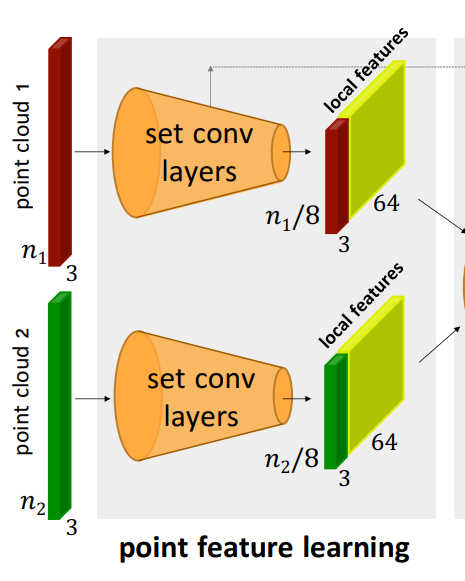
\includegraphics[width=\textwidth,height=0.8\textheight,keepaspectratio]{img/05_FlowNet3D_part1.png}        
        \label{fig:enter-label}
    \end{figure}
    \end{minipage}
    \hfill
    \begin{minipage}{0.45\textwidth}
        Uses PointNet++ architecture
    \end{minipage} 
\end{minipage}
\end{frame}
\begin{frame}[allowframebreaks]
\frametitle{FlowNet3D third part}
\begin{minipage}{\textwidth}
\begin{minipage}{0.45\textwidth}
        \begin{figure}
        \centering        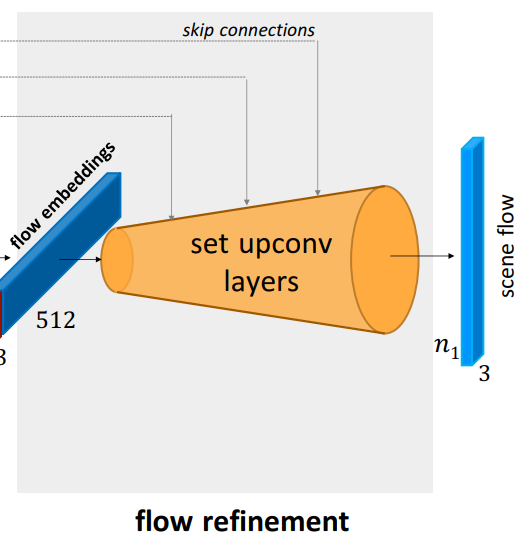
\includegraphics[width=\textwidth,height=0.8\textheight,keepaspectratio]{img/05_FlowNet3D_part3.png}        
        \label{fig:enter-label}
    \end{figure}
    \end{minipage}
    \hfill
    \begin{minipage}{0.45\textwidth}
        Weighs nearby point's features
    \end{minipage} 
\end{minipage}
\end{frame}

\begin{frame}
    \frametitle{Results visualisation}
    \begin{figure}
        \centering
        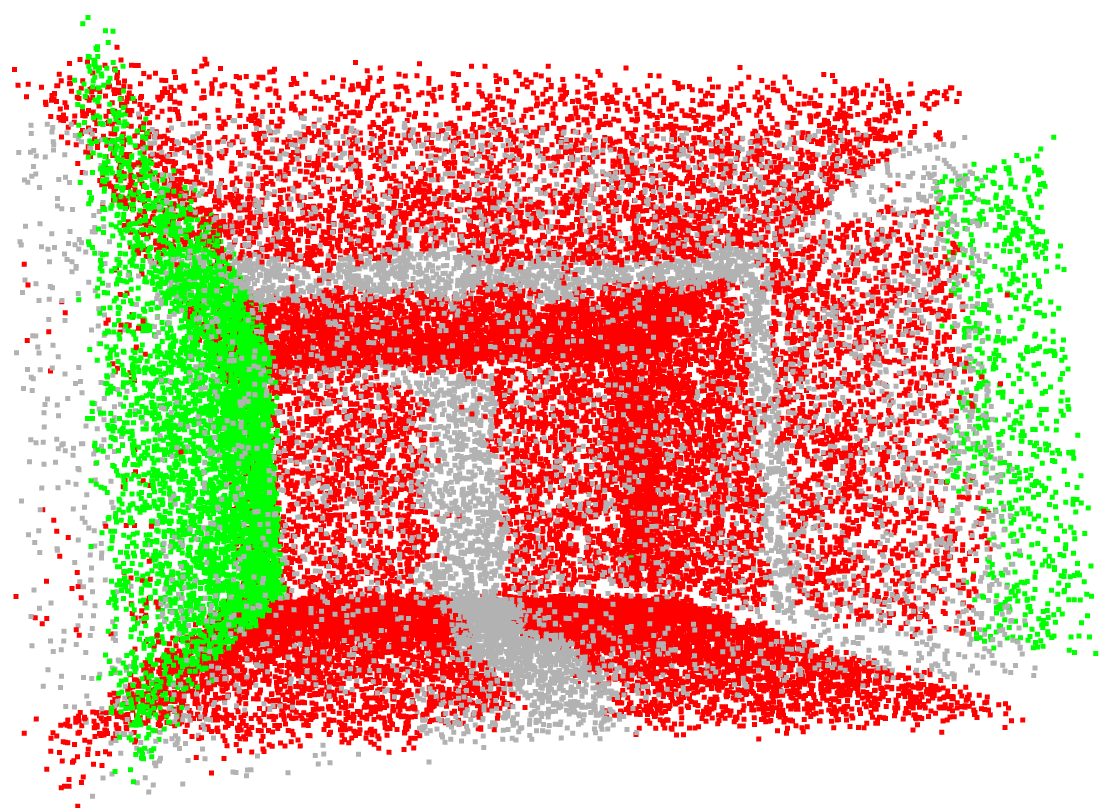
\includegraphics[scale=0.2]{img/Results_gift.png}
        \label{fig:enter-label}
    \end{figure}
\end{frame}

\end{document}

